\section{Context}

Cloud computing is a model for enabling ubiquitous, convenient,
on-demand network access to a shared pool of configurable computing resources
(e.g., networks, servers, storage, applications, and services)
that can be rapidly provisioned and released with minimal management effort or service provider interaction \cite{NIST2011}.
In this model, resources are retrieved from the internet through web-based tools and applications,
rather than a direct connection to a server.
This allows companies to avoid upfront infrastructure costs,
and focus on projects that differentiate their businesses instead of on infrastructure.
Data is stored on physically separate servers and accessed via the internet \cite{Zhang2010}.

There are different kinds of cloud computer.
These types are called `layers', and can be seen in Figure~\ref{figure:layers}.
Starting at the top, the application layer allows the developer to deploy just the functioning application.
The cloud provider will manage everything else.
The bottom layer has all the control with the developer \cite{Zhang2010}.

\begin{center}
    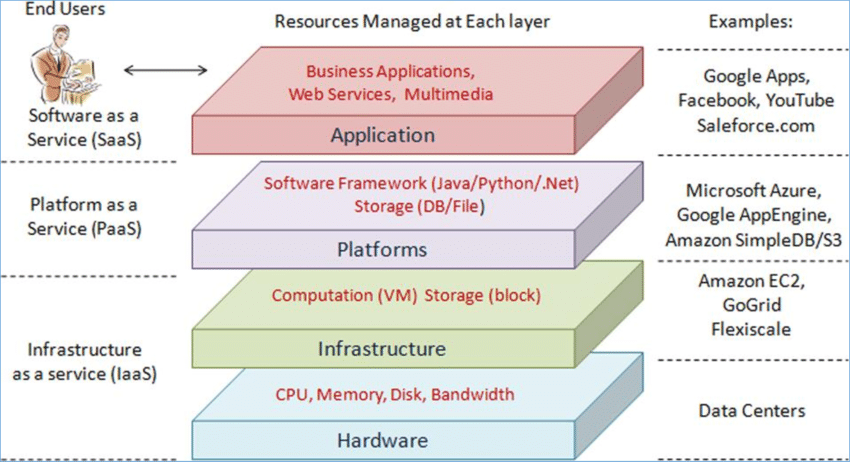
\includegraphics[width=0.4\textwidth]{./graphics/cloud-layers.png}
    \captionof{figure}{Layers of cloud computing}
    \label{figure:layers}
\end{center}

\subsection{Choosing Microsoft Azure}

The cloud computing servers are owned and operated by a third-party cloud service provider,
such as Microsoft Azure, which will be the focus of this research.
The choice for Microsoft Azure was influenced by prior experience with the platform,
its emphasis in cloud computing lectures,
personal preference for Microsoft technology,
and the research's focus on exploring cloud capabilities rather than finding the best provider.

\subsection{Building Blocks}

Cloud providers offer a wide range of services,
each designed to perform a specific function.
These services, or building blocks, cover various categories such as storage,
compute, monitoring, and AI and Machine Learning \cite{Microsoft2023}.
A handfull of examples will be discussed per category.
Please note that these are just examples, and the possibilities are not limited to these options.
These services have been selected since they seem related to the research problem,
even though they might not be selected during the actual research stage.
All the examples are taken from the 2023 article
`Basisprincipes van Azure-toepassingsarchitectuur' by Microsoft \cite{Microsoft2023}.

\subsubsection*{Storage Blocks}

Azure provides several storage options like Azure SQL Database,
Azure Cosmos DB, and Azure Storage Accounts.
These can be used to store the hand-written forms that need to be processed,
as well as the interpreted and processed data.

\begin{itemize}
    \item \textbf{Azure SQL Database}
    \\ This is a fully managed relational database service that provides the broadest SQL Server engine compatibility.

    \item \textbf{Azure Cosmos Database}
    \\ This is a globally distributed,
    multi-model database service for managing data at a large scale with a wide range of APIs including MongoDB.

    \item \textbf{Azure Storage Accounts}
    \\ Provides scalable and secure cloud storage for data, applications, and messaging.
    It`s highly available and durable.
\end{itemize}

\subsubsection*{Compute Blocks}

Azure`s compute services like Azure Virtual Machines,
Azure Functions, Azure Web Apps, Azure Logic Apps,
and Azure API Management can be used to run the applications and processes that interpret and process the hand-written forms.
For example,
an application could be hosted on an Azure Web App that uses an Azure Function to interpret a form when it’s uploaded.

\begin{itemize}
    \item \textbf{Azure Functions}
    \\ A serverless compute service that runs event-triggered code without having to provision or manage infrastructure.

    \item \textbf{Azure Web Apps}
    \\ A service for hosting websites in the cloud. It offers auto-scaling and high availability.

    \item \textbf{Azure Logic Apps}
    \\ A cloud service that helps with automation and orchestration tasks, business processes,
    and workflows when there is a need to integrate apps, data, systems,
    and services across enterprises or organizations.

    \item \textbf{Azure API Management}
    \\ A turnkey solution for publishing APIs to external and internal customers.
\end{itemize}

\subsubsection*{Monitoring Blocks}

Azure’s monitoring services like Azure Monitor and Azure Log Analytics can be used to track the performance of the applications and processes,
helping to identify and resolve any issues that might arise.

\begin{itemize}
    \item \textbf{Azure Monitoring} and \textbf{Azure Log Analytics}
    \\ Collects, analyzes, and acts on telemetry from cloud and on-premises environments.
    It helps to understand how applications are performing and proactively identifies issues affecting them.
\end{itemize}

\subsubsection*{AI and Machine Learning Blocks}

Azure’s AI and Machine Learning services like Azure Cognitive Services can be crucial in interpreting the hand-written forms.
For instance, the Computer Vision OCR could be used to extract text from the hand-written forms,
while Language Understanding (LUIS) and Text Analytics could be used to understand and analyze the extracted text.

\begin{itemize}
    \item \textbf{Language Understanding}
    \\ Allows applications to understand what a person wants in their own words.

    \item \textbf{Text Analytics}
    \\ Detects sentiment, key phrases, named entities, and language from text.

    \item \textbf{Optical Character Recognition}
    \\ Extracts text from images, videos, and more.
\end{itemize}

\subsection{Using Building Blocks}

The building blocks, or services,
provided by Microsoft Azure can be combined and utilized in various ways to address the problem of interpreting,
processing, and confirming hand-written forms.
Microsoft has written a guide that will be followed in designing the solution.
The steps of this guide can be seen in Figure~\ref{figure:design} \cite{Microsoft2023}.

\begin{center}
    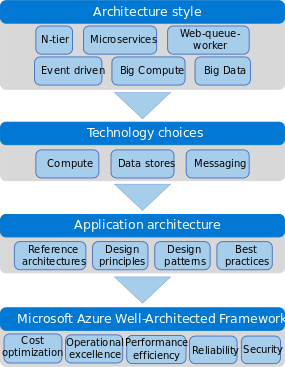
\includegraphics[width=0.4\textwidth]{./graphics/design.png}
    \captionof{figure}{Designing a cloud solution}
    \label{figure:design}
\end{center}